%Write result here
\section{Results}
In this section, we show results of our experiments on the netflix subset dataset. We evaluate our algorithm performance according to the prediction accuracy (using root mean square eror(RMSE) and mean absolute error(MAE) and the number of unpredicted ratings in the test set.

One significant parameter in our algorithm is $K$, number of similar movies to consider in calculating ratings' predictions. We have tried different settings of $K$ to investigate how it can affect the performance of our algorithm. 

%Table \ref{tab:errorsK} summarizes the prediction results for different Ks ranging from to.

%\begin{table}[!ht]
 % \centering
 % \begin{tabular}{|c|c|c|c|}
 %   \hline
 % K & MAE & RMSE & Percentage of Unpredicted Ratings \\
 %   \hline
  %  20 & 0.982 & 1.322 & 30.36\%\\
%\hline
%50 & 0.851 & 1.136 &  12.11\%\\
%\hline
%100 & 0.798 & 1.045 & 5.04 \%
%\hline
%200 & 0.782 & 1.004 & 1.85 \% 
%\hline
%Adaptive &  \\ 
 %   \hline
  %\end{tabular}
  %\caption{Collaborative Filtering (Avg. Ratings) Performance using different $K$ values}
  %\label{tab:errorsK}
%\end{table}
Figure ~\ref{fig:rmse} and Figure \ref{fig:mae} shows the RMSE and MAE for our collaborative filtering algorithm using different values of the number of considered similar movies ($K$). The error measures, RMSE and MAE, are computed for all entries the test set, and for the entries that we could not predict, we use the average rating for the movie under test as our prediction. The average rating per movie is calculated by a pre-processing Map Reduce job. \\

We compare different settings for prediction in Figure ~\ref{fig:rmse} and Figure ~\ref{fig:mae} including: using average rating prediction of the top $K$ movies, using weighted average prediction of the top $K$ movies, and using rounded versions for both average prediction and weighted average prediction. Additionally, we compare our results to two baselines: the first is predicting the global mean of movie ratings for all entries, while the second baseline uses the mean rating of the movie which is being predicted. These mean estimates are calculated using the training ratings only.\\

 It can be observed from Figure \ref{fig:rmse} and Figure \ref{fig:mae} that increasing number of considered similar movies $K$ helps increasing accuracy which is reasonable since increasing $K$ enables our algorithm to predict more missing entries, and accordingly accuracy for these entries increases over the default movie mean rating we have for unpredicted entries. These figures show that using weighted average predictions is slightly better than using average predictions. However, this improvement is slight since we have observed that the variance of cosine similarities between the top $K$ movies being rated by the same user under test is not large. Regarding, rounding the predictions, it can be noticed that rounding reduces MAE while it largely increases RMSE over the movie mean baseline as shown in Figure \ref{fig:rmse} since RMSE is more sensitive than MAE to outliers, so if rounding goes on the wrong direction, RMSE would increase. Accordingly, we have used unrounded version of weighted average prediction for further experiments.


Figure ~\ref{fig:perc} shows the percentage of unpredicted ratings using our collaborative filtering approach as we varies $K$.It can be observed from this figure that increasing $K$ has a significant impact on reducing percentage of unpredicted ratings we have, this is reasonable as considering more similar neighbours (movies), would increase the probability of having some of these movies rated by the users in the test set, and accordingly we can provide more predictions to the missing entries in the test set. However, increasing $K$ beyond some extent would not help much decrease the number of unpredicted entries. Moreover, it could hurt accuracy since we are considering many distant (non-similar) movies if we set $K$ greater than 500 as shown in Figure ~\ref{fig:rmse} and Figure ~\ref{fig:mae} that errors start to saturate or even drop for the MAE at this point. For $K=500$, the percentage of unpredicted ratings is $0.84\%$ and for $K=1000$, the percentage of unpredicted ratings is $0.824\%$. \\
\begin{figure}[!ht]
  \centering
  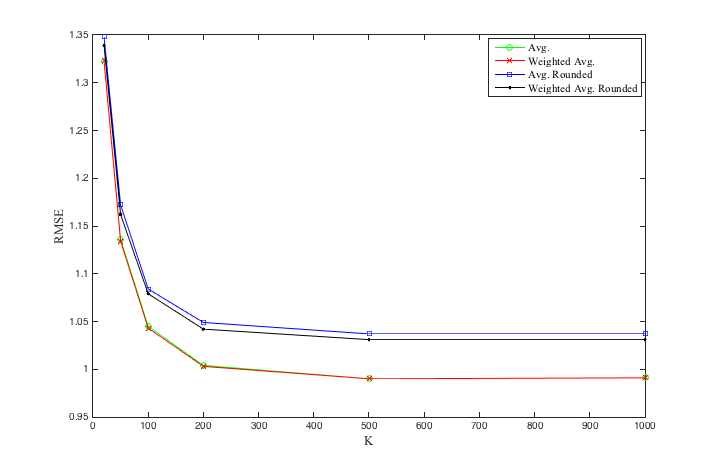
\includegraphics[width=0.8\textwidth]{images/rmse.png}
  \caption{RMSE for our collaborative filtering approach using different $K$ values}
  \label{fig:rmse}
\end{figure}

\begin{figure}[!ht]
  \centering
  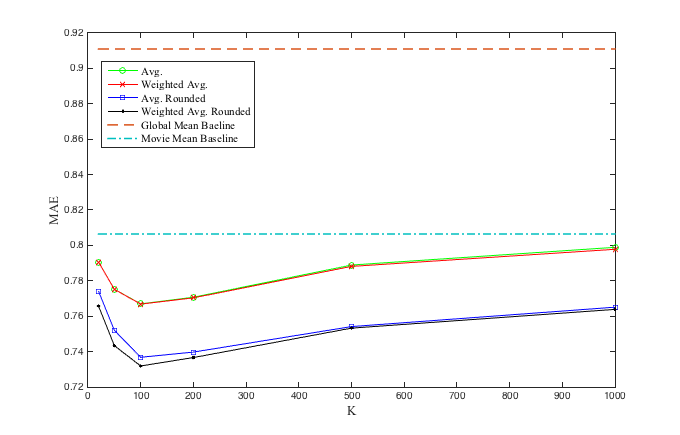
\includegraphics[width=0.8\textwidth]{images/MAE.png}
  \caption{MAE for our collaborative filtering approach using different $K$ values}
  \label{fig:mae}
\end{figure}

\begin{figure}[!ht]
  \centering
  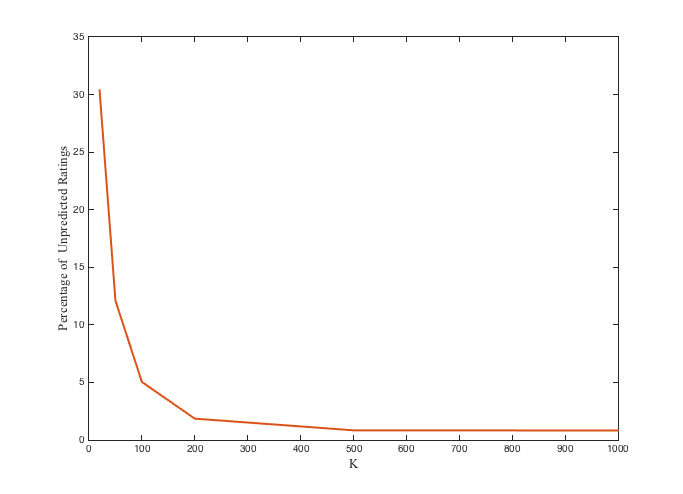
\includegraphics[width=0.7\textwidth]{images/perc.png}
  \caption{Percentage of unpredicted ratings using different $K$ values}
  \label{fig:perc}
\end{figure}

According to our results, increasing $K$ helps improving the overall accuracy, however, for those we can rate using small $K$'s, increasing $K$ would reducer their accuracy since we are considering more distant movies. This can be observed from Figure \ref{fig:rmsepred} which shows the RMSE for the predicted entries only in the test set, excluding the ones that we could not predict using current $K$.
\begin{figure}[!ht]
  \centering
  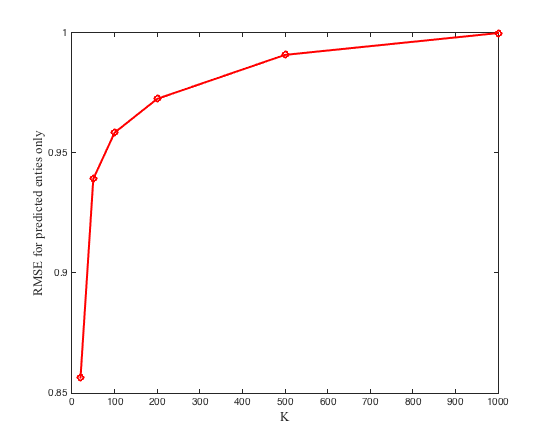
\includegraphics[width=0.8\textwidth]{images/rmsep.png}
  \caption{RMSE using Weighted Avg. Prediction for predicted entries only using different $K$ values}
  \label{fig:rmsepred}
\end{figure}

%%Limiting m
From the results above, we have developed an adaptive prediction scheme that tries to handle both issues of predicting nearly all the missing ratings in the test set, which implies using a large $K$. However, our scheme aims at not sacrificing the accuracy of the already predicted entries , the ones having many overlapping movies that we can predict their ratings with using smaller $K$. Our scheme is to use $K=500$ as it is the best point in terms of both accuracy and percentage of missing ratings $0.84\%$, Figure ~\ref{fig:rmse} and Figure  ~\ref{fig:mae}. However, we limit the number of neighbours (similar movies) actually used in rating prediction to the top $M$ out of these $K$ movies, where $M$ is much less than $K$. \\

Figure ~\ref{fig:rmsem} and ~\ref{fig:maem} show RMSE and MAE for this setting using weighted average predictions, $K=500$ and with variable $M$ from 5 to 100. It can be observed that having too small $M<20$ does not yield the best performance, we think the reason for that can be that some of considered $K$ movies may have only one common user rating them, having 1 cosine similarity, however, such movies with low number of overlapped ratings may not be enough to have accurate predictions. On the other hand increasing $M$ too much would increase the error, this is reasonable and this is the motivation for using $M$. Accordingly, we pick $M=20$, for our final predictions, which was the best point for both Figure ~\ref{fig:rmsem} and ~\ref{fig:maem}.
\begin{figure}[!ht]
  \centering
  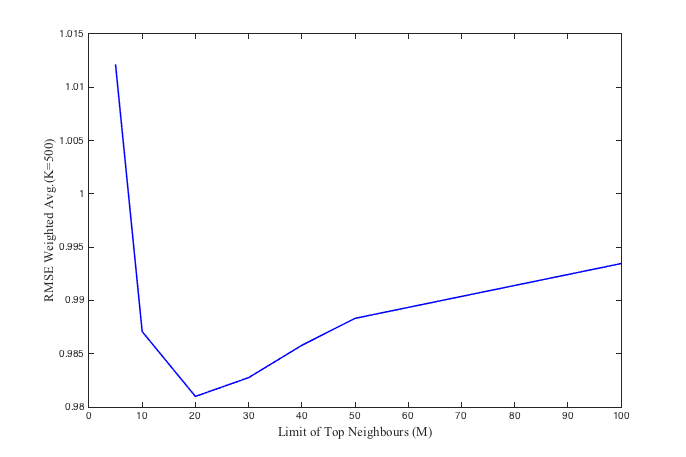
\includegraphics[width=0.8\textwidth]{images/rmsem.png}
  \caption{RMSE using Weighted Avg.  Prediction ($K=500$) using different $M$ values}
  \label{fig:rmsem}
\end{figure}

\begin{figure}[!ht]
  \centering
  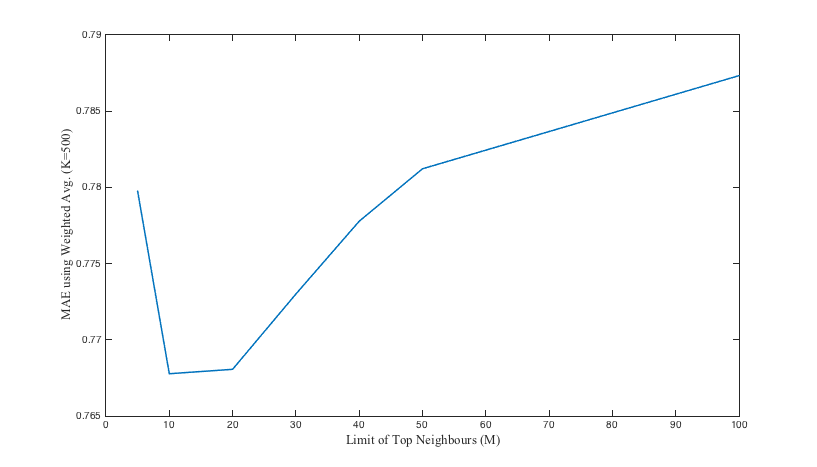
\includegraphics[width=0.8\textwidth]{images/MAEm.png}
  \caption{MAE using Weighted Avg.  Prediction ($K=500$) using different $M$ values}
  \label{fig:maem}
\end{figure}
%%FInal Results Table
Table \ref{tab:finres} summarizes our final results for our developed collaborative filtering approach using $K=500$ and $M=20$. Results are presented in terms of prediction accuracy using RMSE and MAE, and for the number and percentage of predicted ratings that our algorithm was able to make. The table also includes the RMSE and MAE for the two baselines we compare to, the global mean rating and movie mean rating. Table \ref{tab:finres}  shows that our collaborative filtering approach have better accuracy than the two baselines and we almost predict every missing entry.

\begin{table}[!ht]
  \centering
  \begin{tabular}{|c|c|c|c|c|}
    \hline
    Method & RMSE & MAE & Number of Unpredicted Ratings & Percentage of Unpredicted Ratings \\
    \hline
  Collaborative Filtering & \textbf{0.98099}  & \textbf{0.76806} & 841 & 0.84\%\\
\hline
Global Mean Baseline & 1.08502 & 0.91094 & - & - \\
\hline
Movie Mean Baseline & 1.0067 & 0.8065& - &- \\
    \hline
  \end{tabular}
  \caption{Summary of our collaborative filtering and two baselines prediction results}
  \label{tab:finres}
\end{table}


